\documentclass{article}
\usepackage[a4paper,left=3cm, right=3cm, top=2cm, bottom=2cm]{geometry}
\usepackage{amsmath}
\usepackage{graphicx}
\usepackage{caption}
\usepackage{setspace}
\usepackage{xcolor}
\usepackage{titlesec}
\usepackage{amssymb}
\usepackage{tcolorbox}
\usepackage{wrapfig}
\usepackage{amsthm} % For proofs

\graphicspath{{graph/}}
\title{11.8 Definition of Power Series}
\date{}
\author{}
\setstretch{1.3}

% \subsection* 형식 지정 (번호 없음)
\titleformat{name=\section, numberless}
  {\normalfont\large\bfseries\color{blue}}
  {}
  {0pt}
  {}
\geometry{a4paper, margin=1in}

% 증명 환경 스타일
\newtheoremstyle{mystyle}% name
  {}% Space above
  {}% Space below
  {\itshape}% Body font
  {}% Indent amount
  {\bfseries}% Theorem head font
  {.}% Punctuation after theorem head
  {.5em}% Space after theorem head
  {}% Theorem head spec (can be left empty, meaning `normal')
\theoremstyle{mystyle}

\begin{document}
\maketitle

A power series is a type of series that depends on a variable, \(x\). It resembles a polynomial but with infinitely many terms. Power series are central to many applications of calculus, including solving differential equations.

\section*{Definition of Power Series}

\begin{tcolorbox}[
    colback=white,
    colframe=orange!80!white,
    title=Definition of a Power Series,
    boxrule=0.5mm,
    arc=3mm
    ]
    A \textbf{power series} is a series of the form
    \[ \sum_{n=0}^{\infty} c_n x^n = c_0 + c_1 x + c_2 x^2 + c_3 x^3 + \cdots \]
    where \(x\) is a variable and the \(c_n\)'s are constants called the coefficients of the series.
    
    More generally, a series of the form
    \[ \sum_{n=0}^{\infty} c_n (x-a)^n = c_0 + c_1 (x-a) + c_2 (x-a)^2 + \cdots \]
    is called a \textbf{power series centered at \(a\)} or a \textbf{power series about \(a\)}.
\end{tcolorbox}

For a given \(x\), a power series is a series of constants that we can test for convergence or divergence. \\
A power series may converge for some values of \(x\) and diverge for other values. 
\\The sum of the series is a function \( f(x) = \sum_{n=0}^\infty c_n (x-a)^n \) whose domain is the set of all \(x\) for which the series converges. Notice that \(f\) resembles a polynomial.\\
For what values of \(x\) is the series \( \sum_{n=0}^{\infty} x^n \) convergent?\\
This is a geometric series with \(a=1\) and \(r=x\). It converges when \(|x|<1\), that is, for \(-1 < x < 1\). The sum is \( \dfrac{1}{1-x} \).

\subsection*{EXAMPLE 1}
For what values of \(x\) does the series \( \sum_{n=1}^{\infty} \dfrac{(x-3)^n}{n} \) converge?\\
\textbf{SOLUTION:}
Let \(a_n = \dfrac{(x-3)^n}{n}\). We use the Ratio Test.
\begin{align*}
    \lim_{n\to\infty} \left| \dfrac{a_{n+1}}{a_n} \right| &= \lim_{n\to\infty} \left| \dfrac{(x-3)^{n+1}}{n+1} \cdot \dfrac{n}{(x-3)^n} \right| \\
    &= \lim_{n\to\infty} \left| \dfrac{n}{n+1} (x-3) \right| = |x-3| \lim_{n\to\infty} \dfrac{n}{n+1} \\
    &= |x-3| \cdot 1 = |x-3|
\end{align*}
By the Ratio Test, the series converges if \(|x-3| < 1\) and diverges if \(|x-3| > 1\). This means the series converges if \(-1 < x-3 < 1\), which is \(2 < x < 4\). The series diverges if \(x < 2\) or \(x > 4\).

The Ratio Test is inconclusive when \(|x-3| = 1\), so we must test the endpoints \(x=2\) and \(x=4\).
If \(x=4\), the series becomes \( \sum_{n=1}^\infty \dfrac{1^n}{n} = \sum_{n=1}^\infty \dfrac{1}{n} \), the harmonic series, which is divergent.
If \(x=2\), the series becomes \( \sum_{n=1}^\infty \dfrac{(-1)^n}{n} \), which converges by the Alternating Series Test.\\
Thus the given power series converges for \(2 \le x < 4\).

\subsection*{EXAMPLE 2}
For what values of \(x\) is the series \( \sum_{n=0}^{\infty} n! x^n \) convergent?\\
\textbf{SOLUTION:}
We use the Ratio Test. If \(x \neq 0\),
\[ \lim_{n\to\infty} \left| \dfrac{a_{n+1}}{a_n} \right| = \lim_{n\to\infty} \left| \dfrac{(n+1)! x^{n+1}}{n! x^n} \right| = \lim_{n\to\infty} (n+1)|x| = \infty \]
The series diverges for all \(x \neq 0\). When \(x=0\), the series is \( \sum 0 = 0 \), which converges.\\
Thus the series converges only when \(x=0\).

\subsection*{EXAMPLE 3}
For what values of \(x\) does the series \( \sum_{n=1}^{\infty} \dfrac{x^n}{2n!} \) converge?\\
\textbf{SOLUTION:}
Let \(a_n = x^n/2n!\).
\[ \lim_{n\to\infty} \left| \dfrac{a_{n+1}}{a_n} \right| = \lim_{n\to\infty} \left| \dfrac{x^{n+1}}{(2n+2)!} \cdot \dfrac{2n!}{x^n} \right| = \lim_{n\to\infty} \left| \dfrac{x}{n+1} \right| = |x| \lim_{n\to\infty} \dfrac{1}{n+1} = |x| \cdot 0 = 0 \]
Since this limit is 0 for all \(x\), and \(0 < 1\), the series converges for all values of \(x\) by the Ratio Test.\\

\begin{tcolorbox}[
    colback=white,
    colframe=orange!80!white,
    title=Theorem: Convergence of a Power Series,
    boxrule=0.5mm,
    arc=3mm
    ]
    For a given power series \( \sum_{n=0}^{\infty} c_n (x-a)^n \), there are only three possibilities:
    \begin{itemize}
        \item[(i)] The series converges only when \(x=a\).
        \item[(ii)] The series converges for all \(x\).
        \item[(iii)] There is a positive number \(R\) such that the series converges if \(|x-a| < R\) and diverges if \(|x-a| > R\).
    \end{itemize}
    The number \(R\) in case (iii) is called the \textbf{radius of convergence}.\\
    By convention, \(R=0\) in case (i) and \(R=\infty\) in case (ii). \\
    The \textbf{interval of convergence} is the set of values of \(x\) for which the series converges.
\end{tcolorbox}

\begin{figure}[htbp]
    \centering
    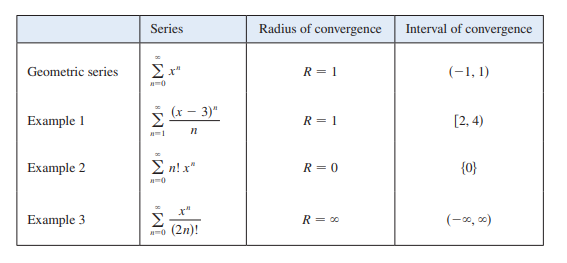
\includegraphics[width=0.8\textwidth]{graph 77.png}
\end{figure}


\subsection*{EXAMPLE 4}
Find the radius of convergence and interval of convergence of the series \( \sum_{n=0}^{\infty} \dfrac{(-3)^n x^n}{\sqrt{n+1}} \).\\
\textbf{SOLUTION:}
Let \(a_n = \dfrac{(-3)^n x^n}{\sqrt{n+1}}\).
\begin{align*}
    \lim_{n\to\infty} \left| \dfrac{a_{n+1}}{a_n} \right| &= \lim_{n\to\infty} \left| \dfrac{(-3)^{n+1} x^{n+1}}{\sqrt{n+2}} \cdot \dfrac{\sqrt{n+1}}{(-3)^n x^n} \right| \\
    &= \lim_{n\to\infty} \left| -3x \sqrt{\dfrac{n+1}{n+2}} \right| = 3|x| \lim_{n\to\infty} \sqrt{\dfrac{1+1/n}{1+2/n}} \\
    &= 3|x| \cdot 1 = 3|x|
\end{align*}
By the Ratio Test, the series converges if \(3|x| < 1\) and diverges if \(3|x| > 1\). Thus it converges if \(|x| < 1/3\) and diverges if \(|x| > 1/3\).
The radius of convergence is \(R = 1/3\).

Now we test the endpoints \(x=1/3\) and \(x=-1/3\).
If \(x=1/3\), the series is \( \sum_{n=0}^\infty \dfrac{(-3)^n (1/3)^n}{\sqrt{n+1}} = \sum_{n=0}^\infty \dfrac{(-1)^n}{\sqrt{n+1}} \). This converges by the Alternating Series Test (\(b_n = 1/\sqrt{n+1}\) is decreasing and approaches 0).\\
If \(x=-1/3\), the series is \( \sum_{n=0}^\infty \dfrac{(-3)^n (-1/3)^n}{\sqrt{n+1}} = \sum_{n=0}^\infty \dfrac{1^n}{\sqrt{n+1}} = \sum_{n=0}^\infty \dfrac{1}{\sqrt{n+1}} \). This is the series \( \sum_{m=1}^\infty 1/\sqrt{m} \) (let \(m=n+1\)), which is a p-series with \(p=1/2 < 1\), so it diverges.

Therefore the interval of convergence is \([-1/3, 1/3)\).

\subsection*{EXAMPLE 5}
Find the radius of convergence and interval of convergence of the series \( \sum_{n=0}^{\infty} \dfrac{n(x+2)^n}{3^{n+1}} \).\\
\textbf{SOLUTION:}
Let \(a_n = \dfrac{n(x+2)^n}{3^{n+1}}\).
\begin{align*}
    \lim_{n\to\infty} \left| \dfrac{a_{n+1}}{a_n} \right| &= \lim_{n\to\infty} \left| \dfrac{(n+1)(x+2)^{n+1}}{3^{n+2}} \cdot \dfrac{3^{n+1}}{n(x+2)^n} \right| \\
    &= \lim_{n\to\infty} \left| \dfrac{n+1}{n} \dfrac{x+2}{3} \right| = \dfrac{|x+2|}{3} \lim_{n\to\infty} \left(1+\dfrac{1}{n}\right) \\
    &= \dfrac{|x+2|}{3}
\end{align*}
Using the Ratio Test, the series converges if \(|x+2|/3 < 1\) and diverges if \(|x+2|/3 > 1\). So it converges if \(|x+2| < 3\).
The radius of convergence is \(R=3\).
The inequality \(|x+2|<3\) can be written \(-3 < x+2 < 3\), which means \(-5 < x < 1\).

We test the endpoints \(x=-5\) and \(x=1\).
If \(x=-5\), the series is \( \sum_{n=0}^\infty \dfrac{n(-3)^n}{3^{n+1}} = \sum_{n=0}^\infty \dfrac{n(-1)^n 3^n}{3 \cdot 3^n} = \dfrac{1}{3} \sum_{n=0}^\infty (-1)^n n \). This series diverges by the Test for Divergence since \( \lim_{n\to\infty} (-1)^n n \) does not exist.\\
If \(x=1\), the series is \( \sum_{n=0}^\infty \dfrac{n(3)^n}{3^{n+1}} = \sum_{n=0}^\infty \dfrac{n 3^n}{3 \cdot 3^n} = \dfrac{1}{3} \sum_{n=0}^\infty n \). This series also diverges by the Test for Divergence since \( \lim_{n\to\infty} n = \infty \).

Therefore the interval of convergence is \((-5, 1)\).

\end{document}